\input{/Users/daniel/github/config/preamble.sty}

\begin{document}

\begin{minipage}{\textwidth}
	\begin{minipage}{1\textwidth}
		Geometry of Algebraic Varieties \hfill Daniel González Casanova Azuela
		
		{\small\hfill\href{https://github.com/danimalabares/ag}{github.com/danimalabares/ag}}
	\end{minipage}
\end{minipage}\vspace{.2cm}\hrule

\vspace{10pt}

{\Huge Exercises in algebraic geometry}

If not explicity stated, exercises are from Hartshorne.

\tableofcontents

\section{Chapter I}

\subsection{No\c c\~oes b\'asicas}

\begin{itemize}
	\item Ussando que $\mathbb{R}=k[x_1,\ldots,x_n]$ \'e Noetheriano (=todo ideal \'e finitamente generado), vimos que todo aberto de Zariski \'e uma uni\~ao finita de conjuntos da forma.

	\item Se $X\subseteq \mathbb{A}^{n} $ \'e uma variedade afim (=existe $\mathfrak{a}\subset R$ tal que $X=\mathbb{V}(\mathfrak{a})$), os conjuntos fechados de $X$ s\~ao $\mathbb{V}(\mathfrak{b})\cap \mathbb{V}(\mathfrak{a})=\mathbb{V}(\mathfrak{a}+\mathfrak{b})$
	
	\item Nullstellenstz fraco:
		\[\operatorname{Spm }(R):=\{\text{ideais maximais de $R$} \} =\{\left<x_1-a_1,\ldots,x_n-a_n\right> :a_i\in k\}\]

	\item Nullstellensatz:
		\[\mathbb{I}(\mathbb{V}(\mathfrak{a}))=\sqrt{\mathbb{a}} \qquad \mathbb{V}(\mathbb{I}(S))=\overline{S}\]

	\item Corol\'ario:

		\[\begin{tikzcd}
			\{\text{affine varieties of $\mathbb{A}^{n} $} \} \arrow[r,"1-1"]&\{\text{radical ideals of $R$} \} \\
			\{\text{irreducible varieties of $\mathbb{A}^{n} $} \}\arrow[r]&\arrow[l]\operatorname{Spec}(R)=\{\text{ideais primos} \} \\
			\{\text{pontos de $\mathbb{A}^{n} $} \} \arrow[r]&\arrow[l]\operatorname{Spm}(R)
		\end{tikzcd}\]
	
	\item Para duas variedades $X\subseteq \mathbb{A}^n$, $Y\subseteq \mathbb{A}^m$,
		\[\operatorname{Hom}(X,Y)=\{\varphi:X\to Y|\exists \tilde{\varphi}=(f_1,\ldots,f_m), f_i\in R \}\]
		e as $f_i$ extendem a $\varphi$.

		 \item Tem uma equival\^encia de categorias
			 \[(\text{affine alg. varieties})^{\operatorname{op}}\to \text{reduced f.g. $k$-algebras}  \]
			 enviando cada variedade $X$ a $R[X]$.

	\item Dimens\~ao de Krull (definida na seç\~ao 3 deste documento), o supremo das alturas de cadeias de ideiais primos, height.

	\item Teorema de Krull.

	\item A imagem de um morfismo n\~ao \'e necessesariamente uma variedade, por\'em, pode pegar o fecho e tudo bem.

	
\end{itemize}

\[D_f=\mathbb{A}^{n} \setminus \mathbb{V}(f).\]

\addcontentsline{toc}{subsection}{Exercise 1.1}
\begin{manualexercise}{1.1}[My first algebraic variety]
	\begin{enumerate}[label*=(\alph*)]\leavevmode
		\item Let $Y$ be the plane curve $y=x^2$ (ie., $Y$ is the zero set of the polynomial $f=y-x^2$). Show that $A(Y)$ is isomorphic to a polynomial ring in one variable over $k$.
		\item Let $Z$ be the plane curve $xy=1$. Show that $A(Z)$ is not isomorphic to a polynomial ring in one variable over $k$.
		\item[*(c)] Let $f$ be any irreducible quadratic polynomial in $k[x,y]$, and let $W$ be the conic defined by $f$. Show that $A(W)$ is isomorphic to $A(Y)$ or $A(Z)$. Which one is it when?
	\end{enumerate}
\end{manualexercise}

\begin{proof}\leavevmode
	\begin{enumerate}[label=(\alph*)]
		\item Consider the map
		\begin{align*}
			k[x,y]&\to k[x]\\
			1&\mapsto1\\
			x&\mapsto x\\
			y&\mapsto x^2
		\end{align*}
		Notice that $y-x^2\in k[x,y]$ is mapped to $0$, so the kernel of this map is $(y-x^2)$. It is also surjective, so we have $A(Y)=k[x,y]/(y-x^2)\cong k[x]$.

	\item In constructing a map like in the former exercise, we may fix $1$ and $x$, and we should map $y$ to $1/x$. However, $1/x$ is not an element of $k[x]$ so we really have an isomorphism $k[x,y]/(xy-1)\cong k[x,\frac{1}{x}]\not\cong k[x]$.

		\item (From \href{https://math.stackexchange.com/questions/2412614/hartshorne-exercise-1-1-c}{StackExchange})
			\begin{enumerate}[label=\textbf{Step \arabic*}]
				\item Factorize the degree 2 homogeneous part into linear factors using that $k$ is algebraically closed.

				\item If these linear factors are linearly dependent,
					\begin{enumerate}
						\item Change coordinates to make the linear factor be the new $X$. The equation becomes $X^2+aX+bY+c$.
						\item Change coordinates to make $aX+bY+Z$ be the new $Y$.
						\item We get $X^2+Y$.
					\end{enumerate}

				\item If these linear factors are linearly independent,
					\begin{enumerate}
						\item Change coordinates to make one of the linear factors be $X$ and the other $Y$. The equation becomes $XY+aX+bY+c$ which can also be written as $(X+a)(Y+b)+d$.
						\item Change the coordinates again to make it $XY+d$.
					\end{enumerate}
			\end{enumerate}
	\end{enumerate}
\end{proof}

\addcontentsline{toc}{subsection}{Exercise 2.14}
\begin{manualexercise}{2.14}[The Segre Embedding]
	Let $\psi:\mathbb{P}^r\times\mathbb{P}^s\to\mathbb{P}^N$ be the map defined by sending the order pair $(a_0,\ldots,a_r)\times(b_0,\ldots,b_s)$ to $(\ldots,a_ib_j,\ldots)$ in lexicographic order, where $N=rs+r+s$. Note that $\psi$ is well-defined and injective. It is called the \textbf{\textit{Segre embedding}}. Show that the image of $\psi$ is a subvariety of $\mathbb{P}^N$. [\textit{Hint}: Let the homogeneous coordinates of $\mathbb{P}^N$ be $\{z_{ij}:i=0,\ldots,r,j=0,\ldots,s\}$ and let $\mathfrak{a}$ be the kernel of the homomorphism $k[\{z_{ij}\}]\to k[x_0,\ldots,x_r,y_0,\ldots,y_s]$ which sends $z_{ij}$ to $x_iy_j$. Then show that $\operatorname{img}\psi=Z(\mathfrak{a})$.
\end{manualexercise}

\begin{proof}[Solution]
	First let's make sure the dimension $N$ is correct. The easy way is found in \href{https://en.wikipedia.org/wiki/Segre_embedding}{wiki}: $N=(r+1)(s+1)-1$ which is the number of possible choices of pairs of things taking one out $r+1$, another out of $s+1$, and then remember there is only one zero index so take one away.
	
	To see that $\psi$ is injective we follow \href{https://math.stackexchange.com/questions/3683364/segre-map-is-an-embedding}{StackExchange}: 
	{\color{azure}Let $z=[z_{00}:z_{01}:\ldots:z_{ij}:\ldots:z_{rs}]$ be an element of the image of $\psi$ and let $(a,b)\in\mathbb{P}^r\times\mathbb{P}^s$ be such that $\psi(a,b)=z$. WLOG we can assume $a_0=b_0=z_{00}=1$. Then $b_j=z_{0j}$ for all $0\leq j\leq s$ and $a_i=z_{i0}$ so $a,b$ are uniquely determined and this map is bijective onto the image.
	
	Actually, what we have done is constructed an inverse morphism of the Segre map. According to StackExchange, this makes it into an embedding.}
	
	To show that $\operatorname{img}\psi$ is a subvariety of $\mathbb{P}^N$ we need to find a set of homogeneous polynomials in $k[z_{ij}]$/
	
	Following the hint, as before let $z\in\operatorname{img}\psi$ and $f$ any polynomial in the kernel of \[k[\{z_{ij}\}]\to k[x_0,\ldots,x_r,y_0,\ldots,y_s]\]. We must show that $f(z)=0$. Well it doesn't make much sense because if $f=\sum a_{ij}z_{ij}$ is in the kernel of that map, then its image $\sum a_{ij}x_iy_j$ is the zero polynomial, so obviously $f(z)=\sum a_{ij}z_{ij}=\sum a_{ij}x_iy_j=0$. So this is confusing.
	
	So what are the equations of $\operatorname{img}\psi$? A polynomial $f(z_{00},\ldots,z_{rs})$ will vanish on $\operatorname{img}\psi$ if somehow it vanishes 
\end{proof}

\addcontentsline{toc}{subsection}{Exercise 2.15}
\begin{manualexercise}{2.15}[The Quadric Surface in $\mathbb{P}^3$]
	Consider the surface $Q$ (a \textbf{\textit{surface}} is a variety of dimension 2) in $\mathbb{P}^3$ defined by the equation $xy-wz=0$.
	\begin{enumerate}
		\item Show that $Q$ is equal to the Segre embedding of $\mathbb{P}^1\times\mathbb{P}^1$ in $\mathbb{P}^3$, for suitable choice of coordinates.
		\item Show that $Q$ contains two families of lines (a \textbf{\textit{line}} is a linear variety of dimension 1), $\{L_t\},\{M_t\}$ each parametrized by $t\in\mathbb{P}^1$, with the properties that if $L_t\neq L_u$ then $L_t\cap L_u=\varnothing$ and if $M_t\neq M_u$, $M_t\cap M_u=\varnothing$, and for all $t,u$, $L_t\cap M_u$ is a point.
		\item Show that $Q$ contains other curves besides these lines, and deduce that the Zariski topology on $Q$ is not homeomorphic via $\psi$ to the product topology on $\mathbb{P}^1\times \mathbb{P}^1$ where each $\mathbb{P}^1$ has its Zariski topology.
	\end{enumerate}
\end{manualexercise}

\begin{proof}[Solution]\leavevmode
	\begin{enumerate}
		\item It turns out that the image of the Segre embedding $\psi:\mathbb{P}^1\times\mathbb{P}^1\to\mathbb{P}^3$ equals is the algebraic variety given by the zeroes of the polynomial $f=z_{00}z_{11}-z_{10}z_{01}\in k[z_{00},z_{01},z_{10},z_{11}]$. One contention is easy: if $(x,y)=([x_0,x_1],[y_0,y_1])\in\operatorname{img}\psi$, then clearly $f(\psi(x,y))=x_0y_0x_1y_1-x_0y_1x_1y_0$ is zero because these are numbers in the field $k$.
		
		Now for the other contention pick $z=[z_{00},z_{01},z_{10},z_{11}]\in V(f)$ and let's find an element $(x,y)\in\mathbb{P}^1\times\mathbb{P}^1$ such that $\psi(x,y)=z$. $z\in V(f)$ means that $z_{00}z_{11}=z_{10}z_{01}$. If $z_{00}\neq0$, then we can define $([z_{00},z_{11}],[z_{01},z_{10}])$ {\color{magenta}what?}
		%so there is always one of $z_{00}$ or $z_{11}$ and one of $z_{10}$ or $z_{01}$ that are not zero.
		
		Maybe for the other contention try to define the inverse map $\operatorname{img}\psi\to\mathbb{P}^1\times\mathbb{P}^1$ by $z=[z_{00},z_{01},z_{10},z_{11}]\mapsto([z_{00},z_{01}],[z_{00},z_{10}])$ when $z_{00}\neq0$ and $([z_{11},z_{01}],[z_{11},z_{10}])$ when $z_{11}\neq0$. Is this defining a global map?
		
		\item The lines correspond to fixing one entry and running over the other one in the Segre embedding $(x,y)\to z$. 
	\end{enumerate}
\end{proof}

\subsection{Summary of section 3}

\begin{defn}[Regular function]
	It is a function from a variety to the field such that at every point there is an open neighbourhood (with respect to the Zariski topology, I guess) such that the function equals the quotient of two polynomials. In the affine case the polynomials are thought as functions on the coordinates of $\mathbb{A}^n$, and in the projective case they must be homogeneous polynomials \textit{of the same degree} (which (apparently) makes the quotient be a well-defined function on $\mathbb{P}^n$, in contrast with general homogeneous polynomials that are not functions).
\end{defn}

Here's a very nice reminder of how homogeneous coordinates work taken from \href{https://en.wikipedia.org/wiki/Homogeneous_coordinates#Introduction}{wiki}:

\begin{enumerate}
\item Any point in the projective plane is represented by a triple $(X,Y,Z)$,  called \textit{\textbf{homogeneous coordinates}} where $X$, $Y$ and $Z$ are not all 0.
	\item The point represented by a given set of homomogeneous coordinates is unchanged if the coordinates are multiplied by a common factor.
		\item Conversely, two sets of homogeneous coordinates represent the samer point if and only if one is obltained from the other by multipliying all the coordinates by the same non-zero constant.
			\item When $Z$ is not 0 the point represented it the point $(X/Z,Y/Z$ in the Euclidean plane.
				\item Whan $Z$ is 0 the point represented is the point at infinity.
					\item (The triple  $(0,0,0)$ does not represent any point. The origin of the Euclidean plane is represented by $(0,0,1)$.
\end{enumerate}

\begin{defn}[Morphism]
	A map between two varieties $\varphi:X\to Y$ is a \textit{\textbf{morphism}} if it pulls back regular functions on $Y$ to regular functions on $X$, ie. if $f:V\subseteq Y\to k$ is regular, then $f\circ \varphi$ is regular too.

	An \textit{\textbf{isomorphism}} is a morphism that admits an inverse morphism.
\end{defn}

\begin{remark}
	An isomorphism must be bijective and bicontinuous but a bijective bicontinuous morphism need not be an isomorphism.
\end{remark}

\begin{defn}[Rings of regular functions]
	$\mathcal{O}(Y)$ is the ring of all regular functions on the variety $Y$ and $\mathcal{O}_P(Y)$ is the \textit{\textbf{local ring}} consisting on functions defined on neighbourhoods of $P\in Y$, any two identified if they coincide near $P$. This is in fact a local ring with maximal ideal the functions that vanish at $P$.
\end{defn}

\begin{prop}[3.5]\leavevmode
	Let $X$ be any variety and let $Y$ be any affine variety. Then there is a natural bijective mappingng of sets
	\[\alpha:\operatorname{Hom}(X,Y)\to \operatorname{Hom}(A(Y),\mathcal{O}(X) \]
	where the left $Hom$ means morphism of varieties and the right  $ \operatorname{Hom}$ means homomorphisms of $k$-algebras.
\end{prop}

	\begin{coro}[3.8]
		The functor $X\mapsto A(X)$ induces an arrow-reversing equivalence of categories between athe category of affine varieties over $k$ and the category of finitely generated integral domains over  $k$.
	\end{coro}

\addcontentsline{toc}{subsection}{Exercise 3.1}
\begin{manualexercise}{3.1}
\begin{enumerate}[label=\alph*.]
	\item Show that any conic in $\mathbb{A}^{2} $ is isomorphic either to $\mathbb{A}^{1} $ or $\mathbb{A}^{1}\setminus \{0\} $.

	\item Show that $\mathbb{A}^{1} $ is not isomorphic to any proper open subset of itself.

	\item Any conic in $\mathbb{P}^2$ is isomorphic to $\mathbb{P}^1$.

	\item We will see later that any two curves are homeomorphic. But show now that $\mathbb{A}^{2} $ is not even homeomorphic to $\mathbb{P}^2$.

	\item If an affine variety is isomorphic to a projective variety, then it consists of only one point.
\end{enumerate}

\begin{proof}[Solution] I understand a \textit{\textbf{conic}} to be zero-set of an (irreducible) quadratic polynomial in either $k[x,y]$ (affine) or in  $S[x,y,z]$.
	\begin{enumerate}[label=\alph*.]
		\item In exercise 1.1 it is shown that any conic in $\mathbb{A}^{2} $ has coordinate ring isomorphic to either $k[x]$ or $k[x,\frac{1}{x}]$. But the coordinate ring of  $\mathbb{A}^{1}\setminus \{0\} $ is not isomorphic to $k[x]$, so we are done.

		\item Notice that an open subset of $\mathbb{A}^{1}$ is $\mathbb{A}^{1} $ minus a finite a set of points, say $a_1,\ldots,a_m$. The coordinate ring of such a variety is $k[x]/(x-a_i)_{i}$, which cannot be isomorphic to $k[x]$. {\color{magenta}I have read that in such a ring $x-a_i$ is a \textit{unit}, while I think it is just zero (the zero class=additive identity).}

		\item \leavevmode 

			\begin{enumerate}[label=\textbf{Step \arabic*}]
				\item Let $f \in k[x,y,z]$ be an irreducible homogeneous polynomial of degree 2. Then  $f$ can be written as $x^{\mathbf{T}}Mx$ with $M$ a $3\times 3$ symmetric matrix. But any such matrix is diagonalizable because $k$ is closed, meaning there is another matrix $Q$ such that $Q^{\mathbf{T}}MQ=D$ with $D$ diagonal.

				\item $Q$ defines a morphism of $\mathbb{P}^n$ to itself since it is composed of linear polynomials (recall that a morphism must pull back regular functions to regular functions, and in the projective case regular functions are locally quotients of homogeneous polynomials of the same degree, so a linear transformation preserves such a structure).

				\item $Q$ restricts to an isomorphism on the zeroes of the initial matrix $M$ and the diagonal matrix $D$, meaning any two conics are isomorphic.

				\item The image of the so-called $2$-uple embedding of $\mathbb{P}^1$ in $\mathbb{P}^2$ is also a conic, so all conics are isomorphic to $\mathbb{P}^1$.
			\end{enumerate}

	\item Algebraic topology.

	\item The ring of regular functions on a projective variety is isomorphic to $k$ by Thm 3.4. But then $A(Y)\cong \mathcal{O}(X)$ by Prop 3.5, which is only true for the coordinate rings of maximal ideals, that correspond to points.

	\end{enumerate}
\end{proof}

\end{manualexercise}

\addcontentsline{toc}{subsection}{Exercise 3.2}
\begin{manualexercise}{3.2}
	A morphism whose underlying map on the topological spaces is a homeomorphism need not be an isomorphism (of algebraic varieties). (Bicontinuous morphism need not be isomorphism.)
	\begin{enumerate}[label=\alph*.]
		\item For example, let $\varphi:\mathbb{A}^1\to \mathbb{A}^2$ be defined by $t\mapsto (t^2,t^3)$. Show that $\varphi$ defines a bicontinuous morphism of $\mathbb{A}^1$ onto the curve $y^2=x^3$, but that $\varphi$ is not an isomorphism.

		\item For another example, let the characteristic of the base field $k$ be $p>0$, and define a map $\varphi:\mathbb{A}^1\to \mathbb{A}^1$ by $t\mapsto t^p$. Show that $\varphi$ is bijective and bicontinuous but not an isomorphism. This is called the \textit{\textbf{Frobenius morphism.}}
	\end{enumerate}
\end{manualexercise}

\begin{proof}[Solution]\leavevmode
	\begin{enumerate}[label=\alph*.]
		\item First notice that $\varphi$ is bijective on its image simply because it is injective.
			\begin{figure}[H]
				\centering
				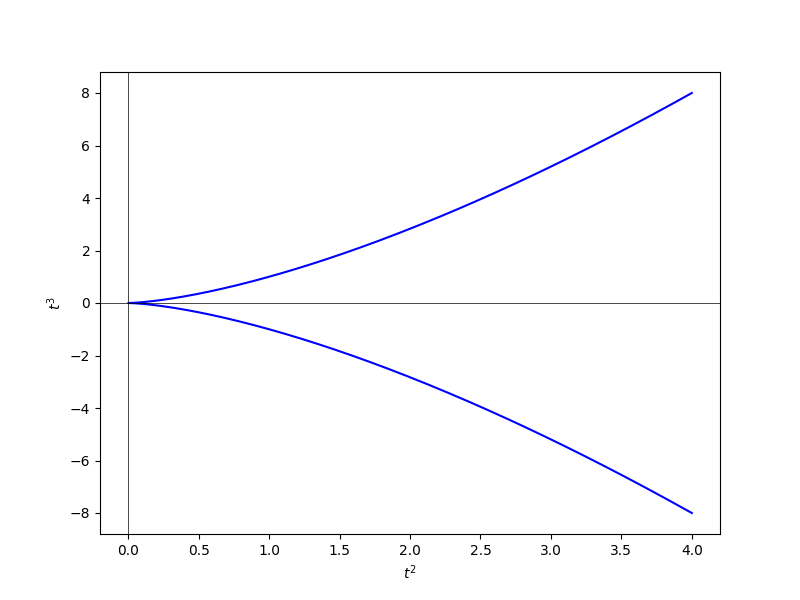
\includegraphics[width=0.5\textwidth]{fig1.png}
			\end{figure}
			
			It is clear that it is a morphism.

			To see if it is continuous first remember that affine space (and also projective space) is equipped with the Zariski topology, whose open sets are complements of algebraic sets (=sets of zeroes of polynomials). But $A=k[x]$ is principal so every algebraic set is the set of zeroes of one polynomial, basically because of this corollary of the Nullstellensatz:
\begin{coro}[[Hart] 1.4]
	There is a one-to-one inclusion-reversing correspondence between algebraic sets in $\mathbb{A}^{n} $ and radical ideals in $k[x_1,\ldots,x_n$ ] (i.e., ideals which are equal to their own radical), given by $Y\mapsto I(Y)$ and $\mathfrak{a}\mapsto Z(\mathfrak{a})$. Furthermore, an algebraic set is irreducible iff its ideal is a prime ideal.
\end{coro}

And $k$ is closed so every polynomial $n$ roots, so algebraic sets are just finite sets.

{\color{magenta}This was seemed relevant at some point…}

\begin{defn}
	The \textit{\textbf{(Krull) dimension}} of a ring $A$ is the supremum of all \textit{\textbf{heights}} of all prime ideals, i.e. the largest proper chain of prime ideals $\mathfrak{p}_0\subset \mathfrak{p}_1\subset\ldots\subset \mathfrak{p}$.
\end{defn}

\begin{prop}[1.7]
	If $Y$ is an affine algebraic set, then the dimension of $Y$ is equal to the dimension of its affine coordinate ring $A(Y)$.
\end{prop}

			We only need to know that closed sets are finite points. This \href{https://math.stackexchange.com/questions/407693/polynomials-are-continuous-with-respect-to-the-zariski-topology}{means} that polynomials are continuous functions with respect to Zariski topology (because preimage of a closed set=finite set of points is closed because it is the root of $p-\alpha$). That makes $\varphi$ continuous.

			Being bicontinuous is the same as being a homeomorphism, which is equivalent to showing that $\varphi$ is open or closed (since we already noted it is bijective). But, finite sets of points are closed sets in the curve (because it is put in affine space---this is not true in general!).

			Finally we show that $\varphi$ is not an isomorphism. Yesterday with Victor we tried to write the inverse map, which should satisfy
\begin{align*}
	 (x,y)&=(\varphi^{-1}(x,y)^2,\varphi^{-1}(x,y)^3)\\
	\implies &\begin{cases}
		\varphi^{-1}(x,y)^2&=x=\frac{x^2}{x^3}=\frac{x^2}{y^2}=\left(\frac{x}{y}\right)^2 \\
		\varphi^{-1}(x,y)^3& =y=\frac{y^2}{y^3}=\frac{x^3}{y^3}=\left(\frac{x}{y}\right)^3
	\end{cases}
\end{align*}
so basically $\varphi^{-1}$ must be $(x,y)\mapsto \frac{x}{y}$ but this is not defined at $y=0$ so I thought well why don't you just put
			\[(x,y)\longmapsto\begin{cases}
				0\qquad &y=0 \\
				\frac{x}{y}\qquad &y\neq 0
			\end{cases}\]
			but then all $(x,0)$ will map to $(0,0)$ under $\varphi\circ \varphi^{-1}$. So what happens is that this map is not well-defined so it is not an isomorphism.

	\item The Frobenius morphism is in fact a ring homomorphism meaining it preserves multiplication and addition. Addition is more \href{https://en.wikipedia.org/wiki/Frobenius_endomorphism#Definition}{interesting}: since $p$ is prime, it divides the numerator and not the denominator of the binomial coefficient $\frac{p!}{k!(p-k)!}$, and this will make that number 0 unless $k=0,n$, which are the first final terms of the binomial expansion  $(a+b)^p$. Therefore we must only show that $\varphi$ has trivial kernel. Now since $k$ is a field, all elements are units, so none of them can actually satisfy $a^p=0$, making $\ker\varphi=0$.

	That $\varphi$ surjective \href{https://en.wikipedia.org/wiki/Perfect_field}{follows} from an equivalence of the field being algebraically closed and thus perfect.

	That $\varphi$ is continuous and bicontinuous follows from the same reasons as the previous question.

	To finish we check that the induced map on coordinates rings is not an isomorphism, since its inverse must be of the form $t\mapsto t^{\frac{1}{p}}$, which is not polynomial.
\end{enumerate}
\end{proof}


\addcontentsline{toc}{subsection}{Exercise 3.16}
\begin{manualexercise}{3.16}[Products of Quasi-Projective Varieties]
	Use the Segre embedding (Ex. 2.14) to identify $\mathbb{P}^n\times\mathbb{P}^m$ with its image and hence give it a structure of projective variety. Now for any two quasi-projective varieties $X\subseteq\mathbb{P}^n$ and $Y\subseteq\mathbb{P}^m$ consider $X\times Y\subseteq\mathbb{P}^n\times\mathbb{P}^m$.
	\begin{enumerate}[label*=(\alph*)]
		\item Show that $X\times Y$ is a quasi-projective variety.
		\item If $X,Y$ are both projective, show that $X\times Y$ is projective.
		\item Show that $X\times Y$ is a product in the category of varieties.
	\end{enumerate}
\end{manualexercise}

\begin{proof}[Solution]
	content...
\end{proof}

\addcontentsline{toc}{subsection}{Exercise 3.17}
\begin{manualexercise}{3.17}
	A variety $Y$ is \textit{\textbf{normal}} ar a point $P\in Y$ if $\mathcal{O}_{P}$ is an integrally closed ring. Y is \textit{\textbf{normal}} if it is normal at every point.
\end{manualexercise}

\addcontentsline{toc}{subsection}{Exercise 3.18}
\begin{manualexercise}{3.18, Projective Normal Varieties}
	A projective variety $Y\subseteq \mathbb{P}^n$ is \textit{\textbf{projectively normal}} (with respect to the given embedding) if its homogeneous coordinate ring $S(Y)$ is integrally closed.

	\begin{defn}
		Let $A\subset B$ be a subring (or a morphism $A\to B$) $b\in B$ is \textit{\textbf{integrally closed}} if it is the root of a polynomial in $A[x]$. Here we mean that  $S(Y)$ equals the set of integrally closed elements with respect to its field of fractions.
	\end{defn}

	\begin{enumerate}[label=\alph*.]
		\item If $Y$ is projectively normal, then $Y$ is normal.

		\item There are normal varieties in projective space which are not projectively normal. For
	\end{enumerate}
\end{manualexercise}

\begin{proof}[Solution]\leavevmode
	\begin{enumerate}[label=\alph*.]
		\item $\forall p \in Y$ and prime ideal $\mathfrak{m}_p  \in\operatorname{Spec}(Y)$ we have
			\[S(Y)\subseteq S(Y)_{\mathfrak{m}_p}\subseteq F(Y)\]
			{\color{magenta}How does this conclude?}

		\item 
	\end{enumerate}
\end{proof}

\section{[Ot] Chapter I: Varieties}

A friend from Cabo Frio just recommended me to have a look at \href{https://www.uio.no/studier/emner/matnat/math/MAT4215/data/masteragbook.pdf}{Ottem\&Ellinsburg, Introduction to Schemes}. Here are some exercises I liked from Chapter 1: Varieties.

\addcontentsline{toc}{subsection}{Exercise 1.5.12}
\begin{manualexercise}{1.5.12}[The diagonal]
	Let $X$ be an affine variety and consider the map
	\begin{align*}
		\Delta: X &\longrightarrow X\times X \\
		x &\longmapsto (x,x)
	\end{align*}
	\begin{enumerate}[label=\alph*.]
		\item Show that $\Delta$ is a polynomial map.
		\item Let $X=\mathbb{A}^{n}(k)$…
		\item …gives an isomorphism $X\to \Delta(X)$. Hint…
	\end{enumerate}
\end{manualexercise}

\addcontentsline{toc}{subsection}{Exercise 1.5.15}
\begin{manualexercise}{1.5.15}
{\color{magenta}Some Lie groups that are algebraic sets}
\end{manualexercise}

\addcontentsline{toc}{subsection}{Exercise 1.5.28}
\begin{manualexercise}{1.5.28}
	Show that the image of the map
	\begin{align*}
		\phi: \mathbb{A}^{1}(k) &\longrightarrow \mathbb{A}^{3}(k) \\
		t &\longmapsto (t^{2},t^{3},t^{6})
	\end{align*}
	is given by $V(x^{3}-y^{2},z-x^{3})$. Show that $\phi$ is bijective. Is $\phi$ an isomorphism of affine varieties.
\end{manualexercise}

\addcontentsline{toc}{subsection}{Exercise 1.5.29}
\begin{manualexercise}{1.5.29}
	Show that the image of the map
	\begin{align*}
		\phi: \mathbb{A}^{1}(k) &\longrightarrow \mathbb{A}^{3}(k) \\
		t &\longmapsto (t^{3},t^{4},t^{5})
	\end{align*}
	is given by $V(x^{4}-y^{3},z^{3}-x^{5},y^{5}-z^{4})$. Show that $\phi$ is bijective. Is $\phi$ an isomorphism of affine varieties.
\end{manualexercise}

\addcontentsline{toc}{subsection}{Exercise 1.5.31}
\begin{manualexercise}{1.5.31}
	Show that the image of the map
	\begin{align*}
		\phi: \mathbb{P}^{1}(k) &\longrightarrow \mathbb{P}^{2}(k) \\
		(x_0:x_1( &\longmapsto (x_0^{2},x_0x_1,x_1^{2})
	\end{align*}
	is given by $V(y_1^{2}-y_0y_2)$. Show that $\phi$ is an isomorphism of projective varieties. Deduce that any projective conic is isomorphic to $\mathbb{P}^{1}(k)$.
\end{manualexercise}

\section{Chapter IV}

\addcontentsline{toc}{subsection}{Exercise 1.2}
\begin{manualexercise}{1.2}[I like this one]
	Again let $X$ be a curve, and let $P_1,\ldots,P_r$ be points. Then there is a rational  function $f\in K(X)$ having poles (of some order) at each of the $P_i$ and regular  elsewhere.  
\end{manualexercise}

\addcontentsline{toc}{subsection}{Exercise 1.7}
\begin{manualexercise}{1.7}[no one]
	A curve $X$ is called \textit{\textbf{hyperelliptic}}…
\end{manualexercise}

\addcontentsline{toc}{subsection}{Exercise 1.8}
\begin{manualexercise}{1.8}[Alex]
	Very useful to know, I think this is done in that book by Bosch of modules,
\end{manualexercise}

\addcontentsline{toc}{subsection}{Exercise 1.9}
\begin{manualexercise}{1.9}[Victor]
	Riemann-Roch for singular curves.
\end{manualexercise}

\addcontentsline{toc}{subsection}{Exercise 2.3(h)}
\begin{manualexercise}{2.3(h)}
	28 bitangents. Remind Sergey.
\end{manualexercise}

\addcontentsline{toc}{subsection}{Exercise 2.5}
\begin{manualexercise}{2.5}
	Prove the theorem of Hurwitz that a curve $X$ of genus $g\geq 2$ over a field of characteristic 0 has at most $84(g-1)$.
\end{manualexercise}

\addcontentsline{toc}{subsection}{Exercise 3.1}
\begin{manualexercise}{3.1}
	If X is a curve of genus 2, show that a divisor D is very ample $\iff \operatorname{deg} D \geq 5$.  This strengthens (3,3.4).
\end{manualexercise}

\addcontentsline{toc}{subsection}{Exercise 3.12}
\begin{manualexercise}{3.12}
	For each value of $d = 2,3,4,5$ and $r$ satisfying $0\leq r\leq \frac{1}{2}(d-1)(d-2)$, show  that there exists an irreducible plane curve of degree d with r nodes and no other  singularities.
\end{manualexercise}

\addcontentsline{toc}{subsection}{Exercise 4.10}
\begin{manualexercise}{4.10}
	If $X$ is an elliptic curve (Sergey: for abelian varieties is also true), show that there is an exact sequence… Picard groups.
\end{manualexercise}

\addcontentsline{toc}{subsection}{Exercise 5.3}
\begin{manualexercise}{5.3}
	Moduli of Curves of Genus 4. The hyperelliptic curves of genus 4 form an irreducible family of dimension 7. The nonhyperelliptic ones form an irreducible  family of dimension 9. The subset of those having only one $g_3^{1}$ is an irreducible  family of dimension 8. [Hint: Use (5.2.2) to count how many complete intersections $Q\cap F_3$ there are.]  
\end{manualexercise}

\addcontentsline{toc}{subsection}{Exercise 6.2}
\begin{manualexercise}{6.2}
	A rational curve of degree 5 in $\mathbb{P}^{3}$ is always contained in a cubic surface, but there  are such curves which are not contained in any quadric surface.  
\end{manualexercise}

\section{Chapter V}

\addcontentsline{toc}{subsection}{Exercise 1.8}
\begin{manualexercise}{1.8}
	Divisor cohomology, neron severi
\end{manualexercise}

\addcontentsline{toc}{subsection}{Exercise 2.8}
\begin{manualexercise}{2.8}
	Locally free sheaves.
\end{manualexercise}

\addcontentsline{toc}{subsection}{Exercise 3.5}
\begin{manualexercise}{3.5}
	5 points in the field, hyperelliptic curve, point at infinity is singular.
\end{manualexercise}

\addcontentsline{toc}{subsection}{Exercise 4.6}
\begin{manualexercise}{4.5}
	
\end{manualexercise}

\addcontentsline{toc}{subsection}{Exercise 4.16}
\begin{manualexercise}{4.16}
	27 lines on Fermat cubic
\end{manualexercise}

\addcontentsline{toc}{subsection}{Exercise 5.1}
\begin{manualexercise}{5.1}
	
\end{manualexercise}

\addcontentsline{toc}{subsection}{Exercise 5.4}
\begin{manualexercise}{5.4}
	
\end{manualexercise}

\addcontentsline{toc}{subsection}{Exercise 5.5}
\begin{manualexercise}{5.5}
	
\end{manualexercise}

\addcontentsline{toc}{subsection}{Exercise 6.2}
\begin{manualexercise}{6.2}[Arthur]
	Beautiful exercise.
\end{manualexercise}

\end{document}
